\documentclass[12pt,twoside]{reedthesis}
    \usepackage{graphicx,latexsym} 
    \usepackage{amssymb,amsthm,amsmath}
    \usepackage{longtable,booktabs,setspace} 
    \usepackage[hyphens]{url}
    \usepackage{rotating}
    \usepackage{natbib}
    % Comment out the natbib line above and uncomment the following two lines to use the new 
    % biblatex-chicago style, for Chicago A. Also make some changes at the end where the 
    % bibliography is included. 
    %\usepackage{biblatex-chicago}
    %\bibliography{thesis}

    \usepackage{graphicx}
    \usepackage{enumitem}
    % \usepackage{times} % other fonts are available like times, bookman, charter, palatino

    \title{My Final College Paper}
    \author{Your R. Name}
    % The month and year that you submit your FINAL draft TO THE LIBRARY (May or December)
    \date{May 200x}
    \division{Mathematics and Natural Sciences}
    \advisor{Advisor F. Name}
    %If you have two advisors for some reason, you can use the following
    %\altadvisor{Your Other Advisor}
    %%% Remember to use the correct department!
    \department{Mathematics}

    \setlength{\parskip}{0pt}
    %%
    %% End Preamble
    %%
    %% The fun begins:
         
         \newenvironment{halfpage}{
             \begin{minipage}{0.5\textwidth}
         }
         {
             \end{minipage}
         }

    \usepackage{braket}
    \usepackage{tristan-math}
    \theoremstyle{definition}\newtheorem{definition}{Definition}
    \theoremstyle{definition}\newtheorem{example}{Example}

    \usetikzlibrary{arrows, shapes.gates.logic.US, calc}


    \newcommand{\TODO}[1]{{ \color{red} \textbf{TODO}: {#1}}}
    \definecolor{background}{HTML}{F0DBB7}
    % \renewcommand{\TODO}[1]{}

% \pagecolor{background}


\begin{document}

\onehalfspacing
\chapter{Quantum Computing}

\section{Learning Problems}

\subsection{A Motivating Example}
Suppose you're involved in a simple card game: A dealer places two cards\footnote{Assume that the cards are either red or black, with equal probability of each occuring}  face down on a table. You win the game and a substantial prize if you can guess whether the two face-down cards share the same color. You're allowed to ask the dealer to reveal cards to you, but for each card revealed your potential prize gets smaller.

How many of the cards do you need to see to determine with certainty whether the cards share the same color? Maybe you don't need to know for certain. How does the probability of you being able to guess the correct answer relate to the number of cards seen?


If you have no information at all, you can't do substantially better (or worse) than a fifty-percent chance. In fact, seeing only a single card, does not give you any more knowledge of what the answer to the question is. If you wanted to know with certainty what the answer was, you would need to see both cards.


This is of course a very simple game, but it is an example of a type of problem that we refer to as \emph{learning problems} or often \emph{oracle problems}. These problems consist of a learner who is trying to determine the answer to some question, generally to find the output of a certain function. The learner starts out with incomplete information, but is given access to an \emph{oracle function} she can query to gain more information. An oracle function--also sometimes called a black-box function--is one that you can evaluate the oracle at any input of your choosing, but you have no information about the function other than its responses to your inputs. The learner's goal is to determine the answer to the question in as few questions as possible.

We rephrase the scenario given above in this language.
Choose 0 to represent a black card and 1 to represent a red card. Suppose the two facedown cards are labeled $a$ and $b$.
\begin{example}
Given oracle access to a function $f: \{a, b\} \rightarrow \{0, 1\}$. What is the minimum number of queries required to determine $f(a) \oplus f(b)$ where $\oplus$ denotes addition mod 2?
\end{example}

Oracle problems are an extremely useful tool classically because they provide a method for determining lower bounds on algorithmic complexity. \textcolor{blue}{Is this true? Expand?}


\begin{example}
    \TODO{Example 2?}
\end{example}


\section{Review of Classical Computation}
    We briefly review some concepts from the classical theory of computation. Throughout this thesis, we will use \emph{digital circuits} as our model of computation.

    Circuits are a way of manipulating logical information. For every concept we discuss here about circuits, there is an analogous concept in propositional logic that encodes the same information. 

    In the same way that we might think of propositional logic as the manipulation of True and False, we think of circuits as the manipulation of bits that are either $0$ or $1$.
    \begin{definition}
        A \emph{bit} is an element $b \in \Z/2\Z$ (define this notation somewhere??). We will express $b$ as either 0 or 1, although at times it may be convenient to think of a bit as true or false. \TODO{Clean up this definition}
    \end{definition}

    
    \TODO{Clean up this whole section}

    We start with the unary gates. These take one bit as input and return one bit. Here is a $\texttt{NOT}$ gate:
    \begin{center}
        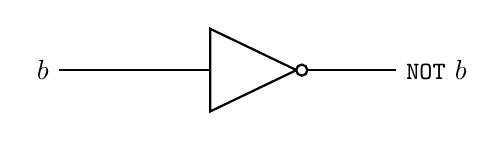
\begin{tikzpicture}[thick]
            \node (b) at (0, 0) {$b$};
            \node (bout) at (5,0) {\texttt{\small NOT} $b$};
            \node[not gate US, draw, minimum size=0.9cm] at ($(b) + (2.5, 0)$) (notb) {};
            \draw (b) -- (notb.input);
            \draw (notb.output) -- (bout);
        \end{tikzpicture}
        
    \end{center}

    It takes 0 to 1 and 1 to 0. It can be defined by the truth table:
    \begin{tabular}{l|l}
    0 & 1 \\
    1 & 0
    \end{tabular}

    There are in fact 4 unary gates, one for each of the 4 truth tables. Writing them out is a good exercise. Importantly More generally, the logic of any circuit is nothing more or less than a truth table. Here is an arbitrary circuit:
    \begin{center}
        \hspace{12mm}
        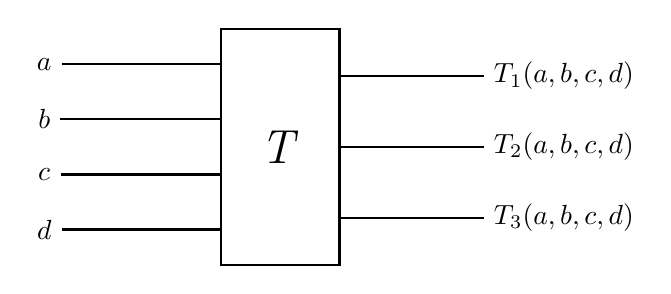
\begin{tikzpicture}[thick]
            \node (a) at (1, 3.05) {$a$};
            \node (b) at (1, 2.35) {$b$};
            \node (c) at (1, 1.65) {$c$};
            \node (d) at (1, 0.95) {$d$};

            \node (x) at (7.6, 2.9) {$T_1(a, b, c, d)$};
            \node (y) at (7.6, 2) {$T_2(a, b, c, d)$};
            \node (z) at (7.6, 1.1) {$T_3(a, b, c, d)$};

            \node (rect) at (4,2) [draw,thick,minimum width=1.5cm,minimum height=3cm] {\textit{\LARGE T}};

            \draw (a) -- (3.24, 3.05);
            \draw (b) -- (3.24, 2.35);
            \draw (c) -- (3.24, 1.65);
            \draw (d) -- (3.24, 0.95);
            \draw (4.76, 2.9) -- (x);
            \draw (4.76, 2) -- (y);
            \draw (4.76, 1.1) -- (z);
        \end{tikzpicture}
    \end{center}
    In this case $T : \{0,1\}^4 \rightarrow \{0,1\}^3$ takes as input 4 bits and returns 3 bits. I use the variable $T$ to emphasize that could be thought of as a truth table.



    There are also two-bit gates, here we have $\texttt{AND}$ and $\texttt{XOR}$. \\

    \begin{halfpage}
        \centering
        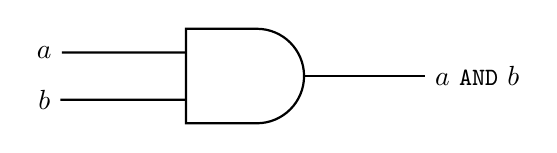
\begin{tikzpicture}[thick]
            \node (x) at (0, 0.8) {$a$};
            \node (y) at (0, 0.2) {$b$};
            \node (output) at (5.5,0.5) {$a$ \texttt{\small AND} $b$};

            \node[and gate US, draw, rotate=0, logic gate inputs=222, minimum size=1.2cm] at ($(2.5, 0.5)$) (xory) {};
            \draw (x) -- (xory.input 1);
            \draw (y) -- (xory.input 3);

            \draw (xory.output) -- (output);
        \end{tikzpicture}
    \end{halfpage}
    \begin{halfpage}
        \centering
        \begin{tikzpicture}[thick]
            \node (x) at (0, 0.8) {$a$};
            \node (y) at (0, 0.2) {$b$};
            \node (output) at (5.5,0.5) {$a$ \oplus \  $b$};


            \node[xor gate US, draw, rotate=0, logic gate inputs=22, minimum size=1.2cm] at ($(2.5, 0.5)$) (xory) {};
            \draw (x) -- (1.74, 0.8);
            \draw (y) -- (1.74, 0.2);

            \draw (xory.output) -- (output);
        \end{tikzpicture}
    \end{halfpage}

    I should mention that you can build any arbitrary circuit using \texttt{AND} and \texttt{NOT}.\,  Here are two examples, \texttt{Controlled AND} and \texttt{Controlled XOR} \\


        \begin{halfpage}
        

        \begin{center}
          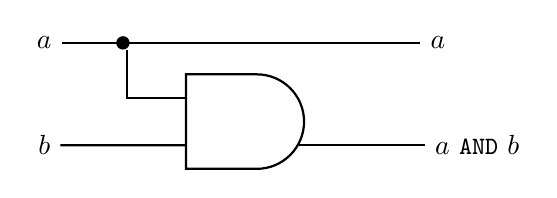
\begin{tikzpicture}[thick]
            \node (x) at (0, 1.5) {$a$};
            \node (y) at (0, 0.2) {$b$};
            \node[circle, fill=black, inner sep=0pt, minimum size=1.7mm] (c) at (1, 1.5) {};
            \node (output) at (5.5,0.2) {$a$ \texttt{\small AND} $b$};
            \node (aout) at (5,1.5){$a$};
     
            \node[and gate US, draw, rotate=0, logic gate inputs=222, minimum size=1.2cm] at ($(2.5, 0.5)$) (xory) {};
            \draw (x) -- (c);
            \draw (c) -- ([xshift=0.4cm]c) |- (xory.input 1);
            \draw (y) -- (xory.input 3);
            \draw (x) -- (aout);
            \draw (3.23,0.2) -- (output);
        \end{tikzpicture}
        \end{center}
        \end{halfpage}
        \begin{halfpage}
        \begin{center}
                \begin{tikzpicture}[thick]
            \node (x) at (0, 1.5) {$a$};
            \node (y) at (0, 0.2) {$b$};
            \node (aout) at (5,1.5){$a$};
            \node (output) at (5.5,0.5) {$a$ \oplus \  $b$};
            \node[circle, fill=black, inner sep=0pt, minimum size=1.7mm] (c) at (1, 1.5) {};

            \node[xor gate US, draw, rotate=0, logic gate inputs=22, minimum size=1.2cm] at ($(2.5, 0.5)$) (xory) {};
            \draw (x) -- (c);
            \draw (c) -- (aout);
            \draw (y) -- (1.74, 0.2);
            \draw (c) -- ([xshift=0.4cm]c) |- (1.74, 0.8);
            \draw (xory.output) -- (output);
        \end{tikzpicture}
        \end{center}
        \end{halfpage}

        The second one, \texttt{Controlled XOR} is $\textit{reversible}$. If we apply it twice, we get the identity.\footnote{Such gates are classically important because they don't add entropy and thus generate less heat. \textcolor{red}{probably remove this}}


        \TODO{Add more information here}


    \subsection{Examples}
        \TODO{Give some simple example of classical circuits and illustrate how the complexity of circuit families is defined}



    \section{Quantum Computation}

    \subsection{Qubits}
    In the same way that classical computation is built out of performing operations on \emph{bits}, quantum computing is built out of performing operations on \emph{qubits}. While a bit can only have two possible states, a qubit lives in a 2-dimensional vector space.

    \begin{definition}
        A \emph{qubit} is a pair of complex numbers
            \[
                (\alpha, \beta) \in \C^2
            \]
        satisfying the normalization condition
        \[
            |\alpha|^2 + |\beta|^2 = 1
        \]
    \end{definition}









    I don't know where I should put this.\footnote{In the literature, quantum states are often defined as living in some generic Hilbert space, instead of identifying it explicitly (in this case as $\C^2$) like we did here. In the general case, we require that every element have norm one. For the purposes of this thesis, we will not need to consider quantum states that cannot be constructed from qubits, so we do not need to worry, but this terminology may be used elsewhere.}



        Importantly, $\C^2$ is a 2-dimensional complex inner-product space. The standard basis vectors form an orthonormal basis for $\C^2$
        \[
            \left\{\cvec{0}{1}, \cvec{1}{0}\right\}
        \]
        \TODO{Explain Diract notation}



        What did I hope to put here?
        We can also have multiple qubit strings. They are expressed as a tensor product. A two qubit string is a vector in $\C^2 \otimes \C^2$ and an $n$ cubit string is a vector in $(\C^2)^{\otimes n}$. This may seem odd, especially if you are not familiar with the tensor product. However, there is good motivation for it. An important property of the tensor product, is that for two vector spaces $V$, $W$
        \[
            \dim (V \otimes W ) = \dim(V)\dim(W)
        \]
        Therefore just as an $n$-bit string has $2^n$ possible states, an $n$-qubit string lives in a $2^n$ dimensional complex vector space. Although we can draw a (limited) picture for one qubit, it quickly becomes impossible even for two qubits.

        \TODO{Explain the tensor product in terms of constructing new basis vectors and extending linearly? Or about the physical interpretation of having two particles with no relationship to each other?}


        \subsection{Quantum Gates and Quantum Circuits}

        \TODO{Make lots of diagrams}

        There is one special qubit operation that is different from the rest, called measurement.

        When we measure a qubit, it ``collapses'' into a classical bit. It becomes $\ket{0}$ with probability $|\alpha|^2$ and $\ket{1}$ with probability $|\beta|^2$. In column vector notation this is

        \[
            \textsf{Measure}\left[\alpha\cvec{0}{1} + \beta\cvec{1}{0}\right] = 
            \begin{cases}
                \cvec{0}{1} &\text{with probability } |\alpha|^2 \vspace{5px}\\
                \cvec{1}{0} &\text{with probability } |\beta|^2
            \end{cases}
        \]

        \TODO{Probably remove this column vector notation}
        \TODO{Introduce POVM measurements}

        \subsection{Quantum Algorithms for Learning Problems}
        Go through examples
        \begin{itemize}
            \item Deutsch-Jozsa simple 2 qubit case 
            \item Bernstein-Vazirani
            \item Grover (as an example of non-sequential queries?)
        \end{itemize}


   \noindent Setup for representation theory and exposition of paper
        \begin{itemize}
            \item Problems where oracles form a group
            \item Coset identification and action of Heisenberg/$GL(2,q) $ as motivation for paper
        \end{itemize}

\chapter{Representation Theory}

\TODO{I'm not really sure what approach I should take to going over the representation theory, I started by just writing out all of the things that I thought were potentially important}

\subsection{\textit{FG}-Modules}
An $F$-vector space $V$ and a group $G$ with a right 
multiplication $m : V \times G \rightarrow V$ satisfying

\begin{enumerate}[label=(\arabic*), topsep=-3px, itemsep=-3px]
    \item $vg \in V$
    \item $v(gh) = (vg)h$
    \item $v1 = v$
    \item $(\alpha v)g = \alpha(vg)$ \ \ \ $\forall \alpha \in F$
    \item $(u + v)g = ug + vg$
\end{enumerate}

\bigskip
\subsection{\textit{FG}-Submodules}
A subset $W$ of an $FG$-module $V$ is an $FG$-\textit{submodule} if 
\begin{enumerate}[label=(\arabic*), topsep=-3px, itemsep=-3px]
    \item $W$ is a vector subspace of $V$
    \item $wg \in W$ \ \  $\forall w\in W,\ g \in G$
\end{enumerate}

\bigskip
\subsection{Irreducibility}
An $FG$-module $V \neq \{0\}$ is said to be \textit{irreducible} if 
it has no $FG$-submodules apart from itself and $\{0\}$. 
A representation $\rho : G \rightarrow \GL(n, F)$ is \textit{irreducible} 
if the corresponding $FG$-module $F^n$ given by $vg = v(g\rho)$ is irreducible. 

The following seems like a useful characterization of irreducibility: \\
Suppose that $V$ is a reducible $FG$-module, so that there 
is an $FG$-submodule $W$ with $0 < \dim(W) < \dim(V)$. Take basis $\mathcal{B}_1$ 
of $W$ and extend it to a basis $\mathcal{B}$ of $V$. 
Then for all $g\in G$, the matrix $[g]_\mathcal{B}$ has the form
    \[
        \begin{bmatrix}
            X_g & 0 \\
            Y_g & Z_g
        \end{bmatrix}
    \]  
for some matrices $X_g$, $Y_g$ and $Z_g$ where $X_g$ is $\dim(W) \times \dim(W)$.
 A representation of degree $n$ is reducible if and only if 
 it is equivalent to a representation of the form above,
where $X_g$ is $k \times k$ and $0 < k <n$.
\bigskip

\subsection{\textit{FG}-Homomorphisms}
Let $V$ and $W$ be $FG$-modules. A function $\varphi : V \rightarrow W$ 
is said to be an $FG$-homomorphism if $\varphi$ is a linear map and 
\[
    (vg)\varphi = (v\varphi)g \quad \forall v\in V,\ g\in G
\]
In other words, if $\varphi$ sends $v$ to $w$ then it sends $vg$ to $wg$.

\bigskip

\subsection{Maschke's Theorem}
Let $G$ be a finite group, let $F$ be $\R$ or $\C$ and let $V$ be an $FG$-module. 
If $U \subseteq V$ is an $FG$-submodule, then there is an $FG$-submodule $W \subseteq V$ such that 
\[
    W = U \oplus W
\]

\subsection{Schur's Lemma}
Let $V$ and $W$ be irreducible \CG-modules
\begin{enumerate}[label=(\arabic*), topsep=-3px, itemsep=-3px]
    \item If $\varphi : V \rightarrow W$ is a \CG-homomorhpism, 
    then either $\varphi$ is an isomorphism, or it maps everything to the identity.
    \item If $\varphi : V \rightarrow V$ is a \CG-ispmorphism, 
    then $\varphi$ is a scalar multiple of the identity morphism $1_V$.
\end{enumerate}

\TODO{Keep going...}


\chapter{Symmetric Oracle Problems}
\TODO{Start this...}


\chapter{Quantum Base Size Examples}

\section{Quantum Base Size of the Heisenberg Group}
\TODO{Sart this}

\section{Quantum Base Size of $\GL(2, q)$}
First we need to understand the representation theory of $\GL(2,q)$

\TODO{This section really needs to be cleaned up and possibly rewritten}
\subsection{Conjugacy classes of $\GL(2,q)$}


Remark that we can trivially represent $GL(2,q) $ as the set of matrices of the form

$$ \begin{bmatrix}
a&b\\
c&d\\
\end{bmatrix}
$$

with determinate $\neq{0}$.\\

Thus a matrix

$$ \begin{bmatrix}
a&b\\
c&d\\
\end{bmatrix}
$$

belongs to $GL(2,q) $ if and only if its rows are linearly independent.  Therefore $(a,b)$ can be anything as long as they are not both zero ($q^2 -1$ choices) and then $(c,d)$ can be anything 
that is not a scalar multiple of $(a,b)$ giving us $q^2-q)$ choices.
Therefore $GL(2,q) $ has $(q^2-q)(q^2-q)$ elements.\\
This argument nice generlizes to $GL(n,q)$.


There are 4 families of conjugacy classes of $G$.
\begin{enumerate}

\item 
$ \begin{bmatrix}
a&b\\
0&d\\
\end{bmatrix}
$
is conjuagte to
$ \begin{bmatrix}
a'&b'\\
0&d'\\
\end{bmatrix}
$
only if $\{a,c\} = \{a',c'\}$ \\
since conjuagate matrices have the same eigenvalues.


The matrices 
\[sI = \begin{bmatrix}
a&b\\
0&d\\
\end{bmatrix}
\]

belong to the center of G.  They give us $q-1$ (the number of choices for s) conjugacy classes of size one.


\item 
Let
\[ g= \begin{bmatrix}
a&b\\
c&d\\
\end{bmatrix}
\in{G}   \textnormal{ and  }    u_s =
\begin{bmatrix}
s&1\\
0&s\\
\end{bmatrix}
\]

Then
\[
gu_s =
\begin{bmatrix}
as&a+bs\\
cs&c+ds\\
\end{bmatrix}
\]

and

\[
u_sg =
\begin{bmatrix}
as&d+bs\\
cs&ds\\
\end{bmatrix}
\]

so $g$ belongs to the centralizer of $u_s$ if and only if $c=0$ and $a=d$.\\
Thus the matrices $u_s$ ($s\in{\mathbb{F}_2}$) give us $q-1$ conjugacy classes.  The order of the centralizer is $(q-1)q$, so by the Orbit-Stabilizer Theorem, each conjugacy class contains $q^2-1$ elements.

\item 
Now let $d_{s,t} =
\begin{bmatrix}
s&0\\
0&t\\
\end{bmatrix}$\\

Note that

$
\begin{bmatrix}
0&1\\
1&0\\
\end{bmatrix}^{-1}
$
$
\begin{bmatrix}
s&0\\
0&t\\
\end{bmatrix}
$
$
\begin{bmatrix}
0&1\\
1&0\\
\end{bmatrix}
$
=
$
\begin{bmatrix}
t&0\\
0&s\\
\end{bmatrix}
$\\

On the other hand, if $\neq{t}$, then we have $gd_{s,t} = d_{s,t}g$ if and only if $b=c=0.$  Thus, the matrices $d_{s,t}$ ($s,t, \in{\mathbb{F}^*_q}, s\neq{t}$) 
give us $/frac{(q-1)(q-2)}{2}$ conjuagacy classes.  The centralizer order is $(q-1)^2$, so again by the orbit-stabalizer theorem each conjugacy class contains $q(q+1)$
elements. 




\item
Finally, consider
$$
v_{r} =
\begin{bmatrix}
    0 & 1 \\
    -r^{1+q} & r + r^2
\end{bmatrix}
\left(
r \in  \mathbb{F}_{q^2}\setminus \mathbb{F}_q
\right)
$$
By our initial proposition $v_r \in G$
\newline
The characteristic polynomial of 
$v_r$
is
$$
\det
(xI - v_r) =
x (x - (r + r^{2}))
+
r^{1 + q}
= (x-r)(x - r^{2})
$$
so $v_{r}$ has eigenvalues of r and $r^{2}$.
\newline
Since $r \notin  \mathbb{F}_{2}$
we see that $v_{r}$ lies in none of the conjegacy classes we have constructed so far.
Now
$$
gv_{r}= 
\begin{bmatrix}
-br^{1+q} & a+b(r+r^{2})\\
-dr^{1+q} & c+d(r+r^{q})
\end{bmatrix}
$$ 
and
$$
v_{r}g= 
\begin{bmatrix}
c  & d\\
-ar^{1+q} +c(r+r^q) & -br^{1+q} + d(r+r^{q})
\end{bmatrix}
$$
Hence
$gv_{r} = v_{r}g$ only if $c = -br^{1+q}$ and $d = a+b(r+r^{2})$
If these conditions hold, then 
$ad-bc = a^{2}+ab(r+r^{2}) + b^{2}r^{1+q} = (a+br) (a+br^{2})$
\newline
Since 
$(a,b) \ne (0,0)$ and $r, r^{q} \notin \mathbb{F}_{q}$ 
we see that $a+br$ and $a+br^{q}$ are non zero.
\newline
Therefore \[
g\in C_{G}(v_{r}) \iff g = 
\begin{bmatrix}
 a & b\\
 -br^{1+q} & a+b(r+r^2)
\end{bmatrix}
\]
\newline 
Thus $|C_G(v_r)| = q^2-1$ and the conjegacy class containing $v_r$ has size $q^2-1$.

\end{enumerate}
\newpage

The matrix $v_t$ has eigenvalues $t$ and $t^q$ so it is not conjugate to $v_r$ unless $t=r$ or $t=r^q$.  
Therefore we can partitian $\mathbb{F}_{q^2}\setminus \mathbb{F}_q$ into subsets of $\{r,r^q\}$.
Each subset gives us a conjugacy class represenative $v_r$ and different subsets give us representatives of different conjugacy classes of G, in fact all of the classes of G.

\subsection*{Conjugacy Classes}
Propostion: There are $q^2-1$ conjugacy classes of $GL(2,q) $ and they are described as follows:

\begin{table}[h]
\begin{tabular}{l|llll}
       &    &    &     &    \\ \hline
class rep  & $sI$ & $u_s$ & $d_{s,t}$ & $v_r$ \\
$|C_G(g)|$     & $(q^2-1)(q^2-q)$  & $(q-1)q$  & $(q-1)^2$   &  $q^2-1$ \\
number of classes & $q-1$ &  $q-1$  & $\frac{(q-1)(q-2)}{2}$   & $\frac{q^2-q}{2}$ 
\end{tabular}
\end{table}


This can be verified by adding to see they sum to the order of the group.









\end{document}